\newpage
\section{Durchführung}
\label{sec:Durchführung}
Mit Hilfe der in Abbildung \ref{fig:Versuchsaufabu} dargestellten Versuchsapperatur sollen zwei
Spektrallinien des Elements Cadium untersucht werden. Dazu wird eine Cd-Lampe mit einem Magnetfeld
durchsetzt und die Änderung der Spektrallinien und ihre Aufspaltung untersucht. Wie aus der Abbildung
bekannt wird nur der transvertale Anteil des Lichts mit Hilfe von Linsen kollimiert.
Das Geradsichtprisma spaltet das Licht in seine spektralen Bestandteile auf.
Mit dem darauf folgenden Spalt und Polarisationsfilters kann die zu untersuchende Spektrallinie ausgewählt werden.
Diese Spektrallinie wird dann auf die Lummer-Gehrcke-Platte fokussiert und erzeugt dort ein Interferenzmuster,
welches mit der Digitalkamera regestriert wird.
Wichtige Kenngrößen sind hier das Dispersionsgebiet
\begin{equation}
    \label{eqn:disp}
    \Delta \lambda_\text{D} = \frac{\lambda^2}{2 \cdot d \sqrt{n^2-1}}
\end{equation}
und das Auflösungsvermögen
\begin{equation}
    \label{eqn:auf}
    A = \frac{\lambda}{\Delta \lambda} = \frac{L \cdot \left(n^2 - 1) \right}{\lambda},
\end{equation}
mit der Wellenlänge $\lambda$, des Brechungsindexes $n$, der Länge der Platte $L$ und der
Dicke der Platte $d$.
\begin{figure}[htb]
  \centering
  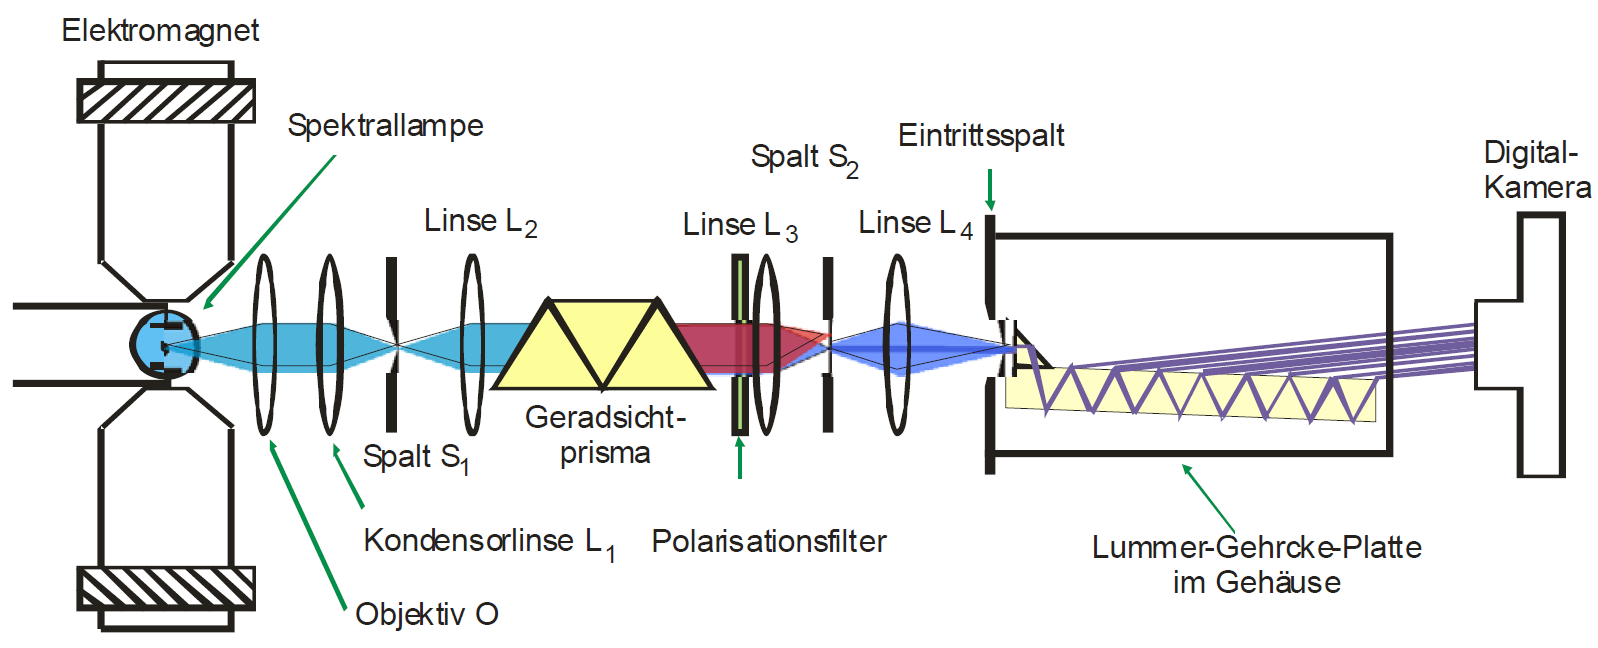
\includegraphics[height=8.0cm]{content/pictures/Versuchsaufbau.png}
  \caption{Schematische Darstellung des verwendeten Versuchsaufbaus. \cite{anleitung_alt}}
  \label{fig:Versuchsaufbau}
\end{figure}
\FloatBarrier